\chapter{Development environment}
\label{chap:devenv}

\section{Development environment overview}

We created a specially configured development environment as a part of our project repository to
simplify the process of the environment setup which is needed to run every integration with our
library and Nussknacker service. For this purpose a separate directory named \texttt{dev-environment} was
created which includes all the Docker configurations and scripts for setting up the environment
from scratch.

The base for configuration for the environment is made of the .env file which contains the environment
constant variables’ definitions and allows easily changing the ports of services and some paths in
Docker images that can be configured. This file is loaded also by the sbt which is then able to work
with the same environment for the purpose of integration tests that use the Docker services to test
every integration.

The process of creating the new environment comes to running a single bash script from the \texttt{dev-environment}
which allows configuring the build process with additional flags specified for script execution. There is
a possibility to run only a single integration environment (e.g. only MLflow server repository with its
environment) or to exclude the process of library recompilation before placing it in the Nussknacker image.
All these improvements were added during the process of adding new integrations as we found it annoying
to spend a lot of time waiting for some part of the environment which wasn’t actually needed to test
and experiment with another integration. Additionally we created the extra bash script for cleaning
the environment cached data as discovered to take a lot of disc space when having so many different
integrations with their environments in a single project.

Every integration has its own \texttt{docker-compose} configuration file which specifies the Docker services
needed to run the integration environment. Additionally, there is a separate configuration named env
for Nussknacker image with its own services, where the compiled Prinz library is placed. Thanks to
such an approach it is easier to set up every environment separately and run only the needed ones.
However this also makes it a little harder to allow communication between every environment - we need
to manually add the Docker network to which the set up environments are connected during creation
time and then can communicate easily. Moreover, we decided not to expose every integration port for
external services for the other integrations and Nussknacker environment but create a single proxy
server for each integration which works as a barrier between the integration implementation details
and the outside world (and then the environment works more like in real life scenario).

The Docker images for each integration needs extra dependencies which are managed using the \texttt{conda}
environment manager. There is quite a lot of work to be done by installing all of them separately
so we decided to create the Docker images for integration and publish it in the external Docker
images repository. We decided to use the GitHub images hub which allows us to publish the images
as a part of our open-source project but unfortunately forces the user to log to GitHub before
downloading the image. However, this GitHub policy can change in the near future as the community
doesn’t seem to like the logging requirement and there are many open discussions on this topic.

\section{Models serving in the environment}

Every integration includes individual ways of models creating and serving them after the training process:

\begin{itemize}
	\item MLflow models are trained after creating the models registry environment and then served as
	Docker services from the same Docker image. Their specification is saved on a separate PostgreSQL
	database and the signatures are kept on the S3 storage provided by the Minio Docker image. This setup
	makes the prepared environment behave like a production version of MLflow server because there is no
	usage of local storage for data keeping.

	\item PMML models are exported as the XML files during training on image start and served as the files
	by the HTTP little server written in Python. This approach uses the PMML Python dependencies only during
	training time as there is no alternative for  models management server in case of PMML models representation.
	The models in our approach have to be listed in a specific way to give the developers ability to
	automatically find their locations with the proper selector path which specifies the models’ refs on the
	main site of the server and is configurable in Prinz.

	\item H2O server is somehow between the MLflow and the PMML integration as it sets up a full models
	registry server during training time and has the ability to list models and serve them with the usage
	of REST API. However in our case the simpler approach to H2O models was chosen and after training the
	models they are saved as the standard MOJO files and then leaded by the Prinz library as the local
	scoring models. Here we leave some room for future integrations as there is also a possibility to
	score the H2O models on the side of the H2O server like in the case of MLflow registry.
\end{itemize}

\section{Proxying models environments}

For each integration we created a separate proxy server based on light nginx alpine Docker image which
is set up with only a single configuration file having needed specifications. In the case of MLflow
integration we tried to simulate the real world scenario usage of MLflow registry by manually setting
the proxy configuration connected with the buffering the data and setting some custom requests’ headers.
In the other integration the served models as the XML and MOJO files are only proxied with the change of
the port on which they are available to the user.

Furthermore, for each integration the proxy also serves a few static files which contain the data needed
in the phase of integration tests. It is responsible for serving like some simple REST API server which
is capable of providing extra inputs for models in specific phases of library tests.

\section{Development environment in integration tests}

Each integration runs separately the integration tests which was one of the main reasons to separate
the environment configurations to a few files. During the tests phase there is a need to know the project
root file in the filesystem to locate these configuration files so before running any integration test
the user has to define the \texttt{REPOSITORY\_ABSOLUTE\_ROOT} environment variable. After this initial
configuration running tests from the console is as simple as calling a single sbt command as the whole
environment configuration is loaded with the sbt plugin from the \texttt{.env} file. However, in the case of need
to run tests from an IDE we need to specify separately the \texttt{.env} file in test run configuration as for now
there is no possibility to load this information automatically in the IDE.

The testing phase includes testing the integration part e.i. scoring the models available in integration
models source and checking their signatures and other parameters. Moreover, there are tests which are
checking the models ability to being proxied with some external data source (outside of Nussknacker
environment source of data) so they use the described feature of nginx serving as a simple REST API
and use the local H2 database as the source of data for tests run. All of these described tests are
wrapped in the abstract traits specifications to allow running them on every integration with the minimal
configuration process. The process of running the tests for specific integration includes setting up the
environment from scratch but everything is done by the testcontainers library which uses the docker-compose
YAML files. This approach connects the source code of our library and its tests with the environment
definition while in the test running phase there is no need for the developer to manually set up the
environment. Additionally, the unit tests which don’t use the integrations’ environment just run scala
tests code without touching anything from the environment definition so there is an easy way to run them
and verify some specified parts of code without the process of working with any Docker containers.

\section{Development environment scheme}

The overview scheme of described development environment is presented below. It shows the scheme of
working with models via Nussknacker's frontend down to models listing and scoring models instances.

\newpage
\scalebox{0.9}{\ifx\du\undefined
  \newlength{\du}
\fi
\setlength{\du}{15\unitlength}
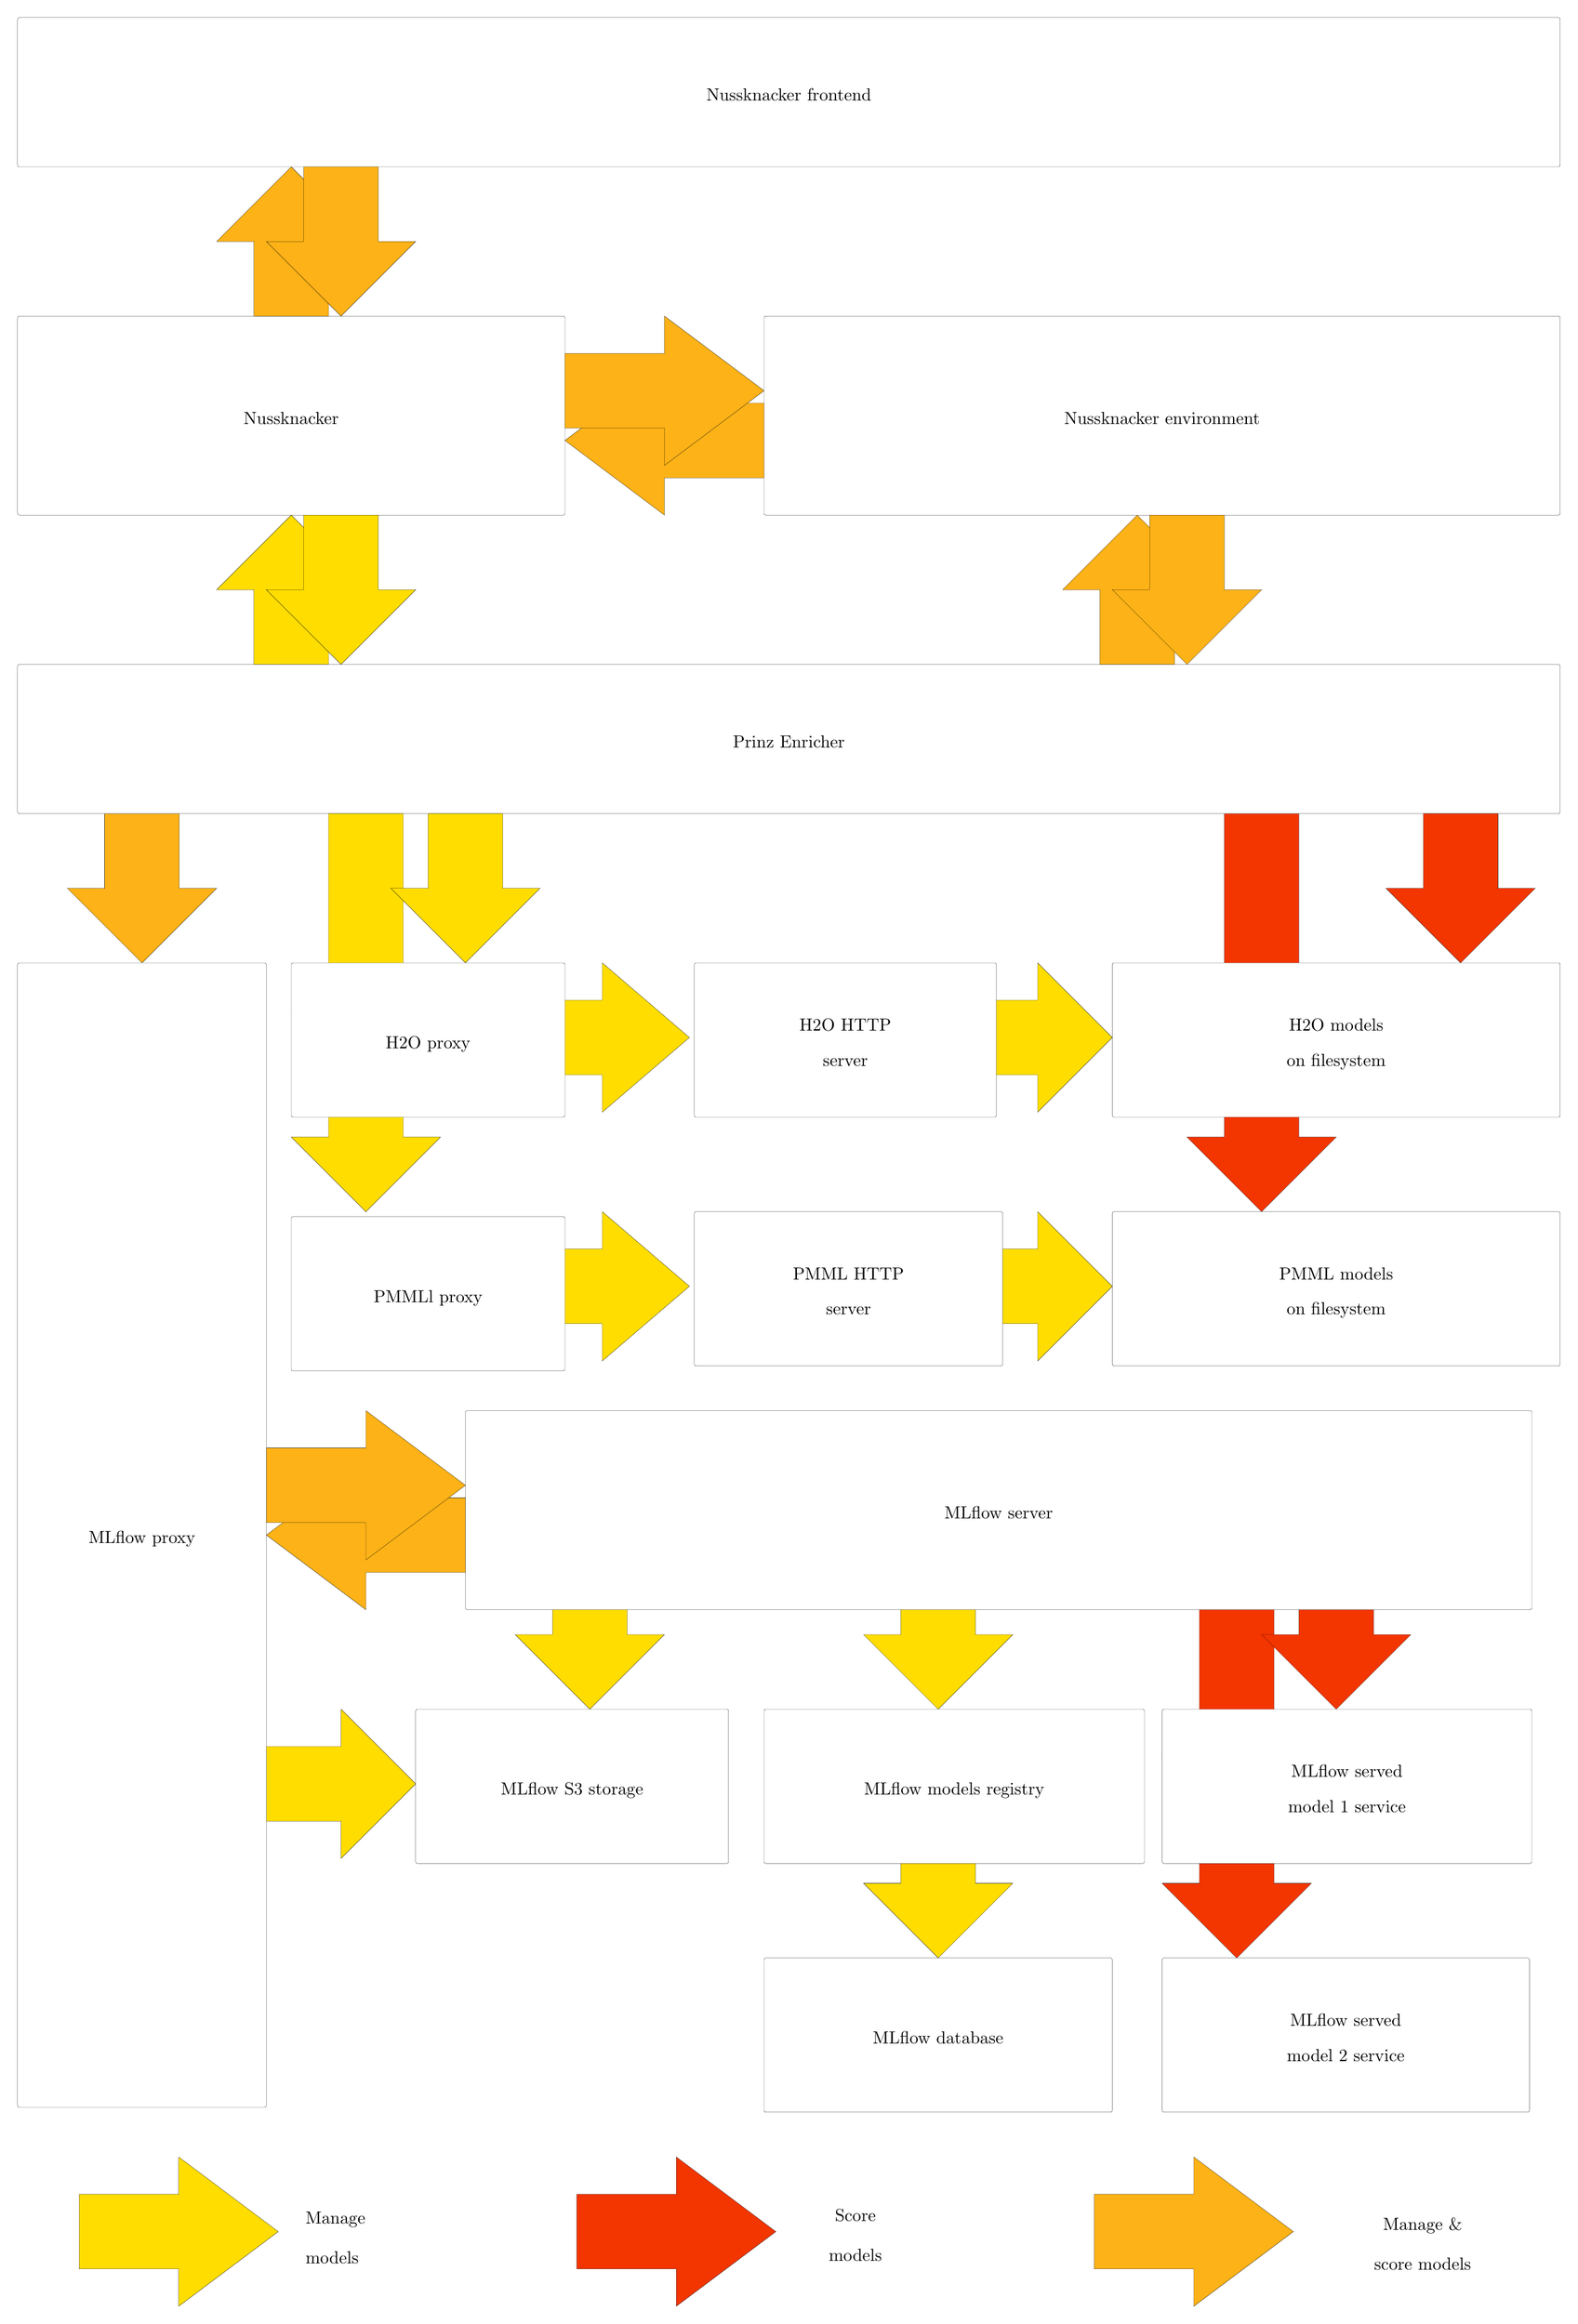
\begin{tikzpicture}[even odd rule]
\pgftransformxscale{1.000000}
\pgftransformyscale{-1.000000}
\definecolor{dialinecolor}{rgb}{0.000000, 0.000000, 0.000000}
\pgfsetstrokecolor{dialinecolor}
\pgfsetstrokeopacity{1.000000}
\definecolor{diafillcolor}{rgb}{1.000000, 1.000000, 1.000000}
\pgfsetfillcolor{diafillcolor}
\pgfsetfillopacity{1.000000}
\pgfsetlinewidth{0.100000\du}
\pgfsetdash{}{0pt}
\pgfsetbuttcap
\pgfsetmiterjoin
\pgfsetlinewidth{0.100000\du}
\pgfsetbuttcap
\pgfsetmiterjoin
\pgfsetdash{}{0pt}
\definecolor{diafillcolor}{rgb}{0.992157, 0.698039, 0.090196}
\pgfsetfillcolor{diafillcolor}
\pgfsetfillopacity{1.000000}
\fill (36.637500\du,52.750000\du)--(38.637500\du,52.750000\du)--(38.637500\du,52.000000\du)--(40.637500\du,53.500000\du)--(38.637500\du,55.000000\du)--(38.637500\du,54.250000\du)--(36.637500\du,54.250000\du)--cycle;
\definecolor{dialinecolor}{rgb}{0.000000, 0.000000, 0.000000}
\pgfsetstrokecolor{dialinecolor}
\pgfsetstrokeopacity{1.000000}
\draw (36.637500\du,52.750000\du)--(38.637500\du,52.750000\du)--(38.637500\du,52.000000\du)--(40.637500\du,53.500000\du)--(38.637500\du,55.000000\du)--(38.637500\du,54.250000\du)--(36.637500\du,54.250000\du)--cycle;
\pgfsetlinewidth{0.100000\du}
\pgfsetdash{}{0pt}
\pgfsetbuttcap
\pgfsetmiterjoin
\pgfsetlinewidth{0.100000\du}
\pgfsetbuttcap
\pgfsetmiterjoin
\pgfsetdash{}{0pt}
\definecolor{diafillcolor}{rgb}{0.952941, 0.207843, 0.000000}
\pgfsetfillcolor{diafillcolor}
\pgfsetfillopacity{1.000000}
\fill (26.237500\du,52.750000\du)--(28.237500\du,52.750000\du)--(28.237500\du,52.000000\du)--(30.237500\du,53.500000\du)--(28.237500\du,55.000000\du)--(28.237500\du,54.250000\du)--(26.237500\du,54.250000\du)--cycle;
\definecolor{dialinecolor}{rgb}{0.000000, 0.000000, 0.000000}
\pgfsetstrokecolor{dialinecolor}
\pgfsetstrokeopacity{1.000000}
\draw (26.237500\du,52.750000\du)--(28.237500\du,52.750000\du)--(28.237500\du,52.000000\du)--(30.237500\du,53.500000\du)--(28.237500\du,55.000000\du)--(28.237500\du,54.250000\du)--(26.237500\du,54.250000\du)--cycle;
\pgfsetlinewidth{0.100000\du}
\pgfsetdash{}{0pt}
\pgfsetbuttcap
\pgfsetmiterjoin
\pgfsetlinewidth{0.100000\du}
\pgfsetbuttcap
\pgfsetmiterjoin
\pgfsetdash{}{0pt}
\definecolor{diafillcolor}{rgb}{1.000000, 0.866667, 0.000000}
\pgfsetfillcolor{diafillcolor}
\pgfsetfillopacity{1.000000}
\fill (16.237500\du,52.750000\du)--(18.237500\du,52.750000\du)--(18.237500\du,52.000000\du)--(20.237500\du,53.500000\du)--(18.237500\du,55.000000\du)--(18.237500\du,54.250000\du)--(16.237500\du,54.250000\du)--cycle;
\definecolor{dialinecolor}{rgb}{0.000000, 0.000000, 0.000000}
\pgfsetstrokecolor{dialinecolor}
\pgfsetstrokeopacity{1.000000}
\draw (16.237500\du,52.750000\du)--(18.237500\du,52.750000\du)--(18.237500\du,52.000000\du)--(20.237500\du,53.500000\du)--(18.237500\du,55.000000\du)--(18.237500\du,54.250000\du)--(16.237500\du,54.250000\du)--cycle;
% setfont left to latex
\definecolor{dialinecolor}{rgb}{0.000000, 0.000000, 0.000000}
\pgfsetstrokecolor{dialinecolor}
\pgfsetstrokeopacity{1.000000}
\definecolor{diafillcolor}{rgb}{0.000000, 0.000000, 0.000000}
\pgfsetfillcolor{diafillcolor}
\pgfsetfillopacity{1.000000}
\node[anchor=base,inner sep=0pt, outer sep=0pt,color=dialinecolor] at (31.837500\du,53.300000\du){Score};
% setfont left to latex
\definecolor{dialinecolor}{rgb}{0.000000, 0.000000, 0.000000}
\pgfsetstrokecolor{dialinecolor}
\pgfsetstrokeopacity{1.000000}
\definecolor{diafillcolor}{rgb}{0.000000, 0.000000, 0.000000}
\pgfsetfillcolor{diafillcolor}
\pgfsetfillopacity{1.000000}
\node[anchor=base,inner sep=0pt, outer sep=0pt,color=dialinecolor] at (31.837500\du,54.100000\du){models};
% setfont left to latex
\definecolor{dialinecolor}{rgb}{0.000000, 0.000000, 0.000000}
\pgfsetstrokecolor{dialinecolor}
\pgfsetstrokeopacity{1.000000}
\definecolor{diafillcolor}{rgb}{0.000000, 0.000000, 0.000000}
\pgfsetfillcolor{diafillcolor}
\pgfsetfillopacity{1.000000}
\node[anchor=base west,inner sep=0pt,outer sep=0pt,color=dialinecolor] at (20.787500\du,53.350000\du){Manage};
% setfont left to latex
\definecolor{dialinecolor}{rgb}{0.000000, 0.000000, 0.000000}
\pgfsetstrokecolor{dialinecolor}
\pgfsetstrokeopacity{1.000000}
\definecolor{diafillcolor}{rgb}{0.000000, 0.000000, 0.000000}
\pgfsetfillcolor{diafillcolor}
\pgfsetfillopacity{1.000000}
\node[anchor=base west,inner sep=0pt,outer sep=0pt,color=dialinecolor] at (20.787500\du,54.150000\du){models};
% setfont left to latex
\definecolor{dialinecolor}{rgb}{0.000000, 0.000000, 0.000000}
\pgfsetstrokecolor{dialinecolor}
\pgfsetstrokeopacity{1.000000}
\definecolor{diafillcolor}{rgb}{0.000000, 0.000000, 0.000000}
\pgfsetfillcolor{diafillcolor}
\pgfsetfillopacity{1.000000}
\node[anchor=base,inner sep=0pt, outer sep=0pt,color=dialinecolor] at (43.237500\du,53.471250\du){Manage \& };
% setfont left to latex
\definecolor{dialinecolor}{rgb}{0.000000, 0.000000, 0.000000}
\pgfsetstrokecolor{dialinecolor}
\pgfsetstrokeopacity{1.000000}
\definecolor{diafillcolor}{rgb}{0.000000, 0.000000, 0.000000}
\pgfsetfillcolor{diafillcolor}
\pgfsetfillopacity{1.000000}
\node[anchor=base,inner sep=0pt, outer sep=0pt,color=dialinecolor] at (43.237500\du,54.271250\du){score models};
\pgfsetlinewidth{0.100000\du}
\pgfsetdash{}{0pt}
\pgfsetbuttcap
\pgfsetmiterjoin
\pgfsetlinewidth{0.100000\du}
\pgfsetbuttcap
\pgfsetmiterjoin
\pgfsetdash{}{0pt}
\definecolor{diafillcolor}{rgb}{0.992157, 0.698039, 0.090196}
\pgfsetfillcolor{diafillcolor}
\pgfsetfillopacity{1.000000}
\fill (16.750000\du,25.000000\du)--(16.750000\du,26.500000\du)--(16.000000\du,26.500000\du)--(17.500000\du,28.000000\du)--(19.000000\du,26.500000\du)--(18.250000\du,26.500000\du)--(18.250000\du,25.000000\du)--cycle;
\definecolor{dialinecolor}{rgb}{0.000000, 0.000000, 0.000000}
\pgfsetstrokecolor{dialinecolor}
\pgfsetstrokeopacity{1.000000}
\draw (16.750000\du,25.000000\du)--(16.750000\du,26.500000\du)--(16.000000\du,26.500000\du)--(17.500000\du,28.000000\du)--(19.000000\du,26.500000\du)--(18.250000\du,26.500000\du)--(18.250000\du,25.000000\du)--cycle;
\pgfsetlinewidth{0.100000\du}
\pgfsetdash{}{0pt}
\pgfsetbuttcap
\pgfsetmiterjoin
\pgfsetlinewidth{0.100000\du}
\pgfsetbuttcap
\pgfsetmiterjoin
\pgfsetdash{}{0pt}
\definecolor{diafillcolor}{rgb}{0.952941, 0.207843, 0.000000}
\pgfsetfillcolor{diafillcolor}
\pgfsetfillopacity{1.000000}
\fill (39.250000\du,25.000000\du)--(39.250000\du,29.000000\du)--(38.500000\du,29.000000\du)--(40.000000\du,33.000000\du)--(41.500000\du,29.000000\du)--(40.750000\du,29.000000\du)--(40.750000\du,25.000000\du)--cycle;
\definecolor{dialinecolor}{rgb}{0.000000, 0.000000, 0.000000}
\pgfsetstrokecolor{dialinecolor}
\pgfsetstrokeopacity{1.000000}
\draw (39.250000\du,25.000000\du)--(39.250000\du,29.000000\du)--(38.500000\du,29.000000\du)--(40.000000\du,33.000000\du)--(41.500000\du,29.000000\du)--(40.750000\du,29.000000\du)--(40.750000\du,25.000000\du)--cycle;
\pgfsetlinewidth{0.100000\du}
\pgfsetdash{}{0pt}
\pgfsetbuttcap
\pgfsetmiterjoin
\pgfsetlinewidth{0.100000\du}
\pgfsetbuttcap
\pgfsetmiterjoin
\pgfsetdash{}{0pt}
\definecolor{diafillcolor}{rgb}{0.952941, 0.207843, 0.000000}
\pgfsetfillcolor{diafillcolor}
\pgfsetfillopacity{1.000000}
\fill (39.250000\du,30.000000\du)--(39.250000\du,31.500000\du)--(38.500000\du,31.500000\du)--(40.000000\du,33.000000\du)--(41.500000\du,31.500000\du)--(40.750000\du,31.500000\du)--(40.750000\du,30.000000\du)--cycle;
\definecolor{dialinecolor}{rgb}{0.000000, 0.000000, 0.000000}
\pgfsetstrokecolor{dialinecolor}
\pgfsetstrokeopacity{1.000000}
\draw (39.250000\du,30.000000\du)--(39.250000\du,31.500000\du)--(38.500000\du,31.500000\du)--(40.000000\du,33.000000\du)--(41.500000\du,31.500000\du)--(40.750000\du,31.500000\du)--(40.750000\du,30.000000\du)--cycle;
\pgfsetlinewidth{0.100000\du}
\pgfsetdash{}{0pt}
\pgfsetmiterjoin
{\pgfsetcornersarced{\pgfpoint{1.000000\du}{1.000000\du}}\definecolor{diafillcolor}{rgb}{1.000000, 1.000000, 1.000000}
\pgfsetfillcolor{diafillcolor}
\pgfsetfillopacity{1.000000}
\fill (23.000000\du,43.000000\du)--(23.000000\du,46.100000\du)--(29.287500\du,46.100000\du)--(29.287500\du,43.000000\du)--cycle;
}{\pgfsetcornersarced{\pgfpoint{1.000000\du}{1.000000\du}}\definecolor{dialinecolor}{rgb}{0.000000, 0.000000, 0.000000}
\pgfsetstrokecolor{dialinecolor}
\pgfsetstrokeopacity{1.000000}
\draw (23.000000\du,43.000000\du)--(23.000000\du,46.100000\du)--(29.287500\du,46.100000\du)--(29.287500\du,43.000000\du)--cycle;
}% setfont left to latex
\definecolor{dialinecolor}{rgb}{0.000000, 0.000000, 0.000000}
\pgfsetstrokecolor{dialinecolor}
\pgfsetstrokeopacity{1.000000}
\definecolor{diafillcolor}{rgb}{0.000000, 0.000000, 0.000000}
\pgfsetfillcolor{diafillcolor}
\pgfsetfillopacity{1.000000}
\node[anchor=base,inner sep=0pt, outer sep=0pt,color=dialinecolor] at (26.143750\du,44.722222\du){MLflow S3 storage};
\pgfsetlinewidth{0.100000\du}
\pgfsetdash{}{0pt}
\pgfsetmiterjoin
{\pgfsetcornersarced{\pgfpoint{1.000000\du}{1.000000\du}}\definecolor{diafillcolor}{rgb}{1.000000, 1.000000, 1.000000}
\pgfsetfillcolor{diafillcolor}
\pgfsetfillopacity{1.000000}
\fill (30.000000\du,48.000000\du)--(30.000000\du,51.100000\du)--(37.000000\du,51.100000\du)--(37.000000\du,48.000000\du)--cycle;
}{\pgfsetcornersarced{\pgfpoint{1.000000\du}{1.000000\du}}\definecolor{dialinecolor}{rgb}{0.000000, 0.000000, 0.000000}
\pgfsetstrokecolor{dialinecolor}
\pgfsetstrokeopacity{1.000000}
\draw (30.000000\du,48.000000\du)--(30.000000\du,51.100000\du)--(37.000000\du,51.100000\du)--(37.000000\du,48.000000\du)--cycle;
}% setfont left to latex
\definecolor{dialinecolor}{rgb}{0.000000, 0.000000, 0.000000}
\pgfsetstrokecolor{dialinecolor}
\pgfsetstrokeopacity{1.000000}
\definecolor{diafillcolor}{rgb}{0.000000, 0.000000, 0.000000}
\pgfsetfillcolor{diafillcolor}
\pgfsetfillopacity{1.000000}
\node[anchor=base,inner sep=0pt, outer sep=0pt,color=dialinecolor] at (33.500000\du,49.722222\du){MLflow database};
\pgfsetlinewidth{0.100000\du}
\pgfsetdash{}{0pt}
\pgfsetbuttcap
\pgfsetmiterjoin
\pgfsetlinewidth{0.100000\du}
\pgfsetbuttcap
\pgfsetmiterjoin
\pgfsetdash{}{0pt}
\definecolor{diafillcolor}{rgb}{1.000000, 0.866667, 0.000000}
\pgfsetfillcolor{diafillcolor}
\pgfsetfillopacity{1.000000}
\fill (32.750000\du,45.000000\du)--(32.750000\du,46.500000\du)--(32.000000\du,46.500000\du)--(33.500000\du,48.000000\du)--(35.000000\du,46.500000\du)--(34.250000\du,46.500000\du)--(34.250000\du,45.000000\du)--cycle;
\definecolor{dialinecolor}{rgb}{0.000000, 0.000000, 0.000000}
\pgfsetstrokecolor{dialinecolor}
\pgfsetstrokeopacity{1.000000}
\draw (32.750000\du,45.000000\du)--(32.750000\du,46.500000\du)--(32.000000\du,46.500000\du)--(33.500000\du,48.000000\du)--(35.000000\du,46.500000\du)--(34.250000\du,46.500000\du)--(34.250000\du,45.000000\du)--cycle;
\pgfsetlinewidth{0.100000\du}
\pgfsetdash{}{0pt}
\pgfsetbuttcap
\pgfsetmiterjoin
\pgfsetlinewidth{0.100000\du}
\pgfsetbuttcap
\pgfsetmiterjoin
\pgfsetdash{}{0pt}
\definecolor{diafillcolor}{rgb}{0.952941, 0.207843, 0.000000}
\pgfsetfillcolor{diafillcolor}
\pgfsetfillopacity{1.000000}
\fill (38.750000\du,40.000000\du)--(38.750000\du,44.000000\du)--(38.000000\du,44.000000\du)--(39.500000\du,48.000000\du)--(41.000000\du,44.000000\du)--(40.250000\du,44.000000\du)--(40.250000\du,40.000000\du)--cycle;
\definecolor{dialinecolor}{rgb}{0.000000, 0.000000, 0.000000}
\pgfsetstrokecolor{dialinecolor}
\pgfsetstrokeopacity{1.000000}
\draw (38.750000\du,40.000000\du)--(38.750000\du,44.000000\du)--(38.000000\du,44.000000\du)--(39.500000\du,48.000000\du)--(41.000000\du,44.000000\du)--(40.250000\du,44.000000\du)--(40.250000\du,40.000000\du)--cycle;
\pgfsetlinewidth{0.100000\du}
\pgfsetdash{}{0pt}
\pgfsetbuttcap
\pgfsetmiterjoin
\pgfsetlinewidth{0.100000\du}
\pgfsetbuttcap
\pgfsetmiterjoin
\pgfsetdash{}{0pt}
\definecolor{diafillcolor}{rgb}{0.952941, 0.207843, 0.000000}
\pgfsetfillcolor{diafillcolor}
\pgfsetfillopacity{1.000000}
\fill (38.750000\du,45.000000\du)--(38.750000\du,46.500000\du)--(38.000000\du,46.500000\du)--(39.500000\du,48.000000\du)--(41.000000\du,46.500000\du)--(40.250000\du,46.500000\du)--(40.250000\du,45.000000\du)--cycle;
\definecolor{dialinecolor}{rgb}{0.000000, 0.000000, 0.000000}
\pgfsetstrokecolor{dialinecolor}
\pgfsetstrokeopacity{1.000000}
\draw (38.750000\du,45.000000\du)--(38.750000\du,46.500000\du)--(38.000000\du,46.500000\du)--(39.500000\du,48.000000\du)--(41.000000\du,46.500000\du)--(40.250000\du,46.500000\du)--(40.250000\du,45.000000\du)--cycle;
\pgfsetlinewidth{0.100000\du}
\pgfsetdash{}{0pt}
\pgfsetmiterjoin
{\pgfsetcornersarced{\pgfpoint{1.000000\du}{1.000000\du}}\definecolor{diafillcolor}{rgb}{1.000000, 1.000000, 1.000000}
\pgfsetfillcolor{diafillcolor}
\pgfsetfillopacity{1.000000}
\fill (38.000000\du,43.000000\du)--(38.000000\du,46.100000\du)--(45.431875\du,46.100000\du)--(45.431875\du,43.000000\du)--cycle;
}{\pgfsetcornersarced{\pgfpoint{1.000000\du}{1.000000\du}}\definecolor{dialinecolor}{rgb}{0.000000, 0.000000, 0.000000}
\pgfsetstrokecolor{dialinecolor}
\pgfsetstrokeopacity{1.000000}
\draw (38.000000\du,43.000000\du)--(38.000000\du,46.100000\du)--(45.431875\du,46.100000\du)--(45.431875\du,43.000000\du)--cycle;
}% setfont left to latex
\definecolor{dialinecolor}{rgb}{0.000000, 0.000000, 0.000000}
\pgfsetstrokecolor{dialinecolor}
\pgfsetstrokeopacity{1.000000}
\definecolor{diafillcolor}{rgb}{0.000000, 0.000000, 0.000000}
\pgfsetfillcolor{diafillcolor}
\pgfsetfillopacity{1.000000}
\node[anchor=base,inner sep=0pt, outer sep=0pt,color=dialinecolor] at (41.715938\du,44.369444\du){MLflow served };
% setfont left to latex
\definecolor{dialinecolor}{rgb}{0.000000, 0.000000, 0.000000}
\pgfsetstrokecolor{dialinecolor}
\pgfsetstrokeopacity{1.000000}
\definecolor{diafillcolor}{rgb}{0.000000, 0.000000, 0.000000}
\pgfsetfillcolor{diafillcolor}
\pgfsetfillopacity{1.000000}
\node[anchor=base,inner sep=0pt, outer sep=0pt,color=dialinecolor] at (41.715938\du,45.075000\du){model 1 service};
\pgfsetlinewidth{0.100000\du}
\pgfsetdash{}{0pt}
\pgfsetbuttcap
\pgfsetmiterjoin
\pgfsetlinewidth{0.100000\du}
\pgfsetbuttcap
\pgfsetmiterjoin
\pgfsetdash{}{0pt}
\definecolor{diafillcolor}{rgb}{0.952941, 0.207843, 0.000000}
\pgfsetfillcolor{diafillcolor}
\pgfsetfillopacity{1.000000}
\fill (40.750000\du,40.000000\du)--(40.750000\du,41.500000\du)--(40.000000\du,41.500000\du)--(41.500000\du,43.000000\du)--(43.000000\du,41.500000\du)--(42.250000\du,41.500000\du)--(42.250000\du,40.000000\du)--cycle;
\definecolor{dialinecolor}{rgb}{0.000000, 0.000000, 0.000000}
\pgfsetstrokecolor{dialinecolor}
\pgfsetstrokeopacity{1.000000}
\draw (40.750000\du,40.000000\du)--(40.750000\du,41.500000\du)--(40.000000\du,41.500000\du)--(41.500000\du,43.000000\du)--(43.000000\du,41.500000\du)--(42.250000\du,41.500000\du)--(42.250000\du,40.000000\du)--cycle;
\pgfsetlinewidth{0.100000\du}
\pgfsetdash{}{0pt}
\pgfsetmiterjoin
{\pgfsetcornersarced{\pgfpoint{1.000000\du}{1.000000\du}}\definecolor{diafillcolor}{rgb}{1.000000, 1.000000, 1.000000}
\pgfsetfillcolor{diafillcolor}
\pgfsetfillopacity{1.000000}
\fill (38.000000\du,48.000000\du)--(38.000000\du,51.100000\du)--(45.381875\du,51.100000\du)--(45.381875\du,48.000000\du)--cycle;
}{\pgfsetcornersarced{\pgfpoint{1.000000\du}{1.000000\du}}\definecolor{dialinecolor}{rgb}{0.000000, 0.000000, 0.000000}
\pgfsetstrokecolor{dialinecolor}
\pgfsetstrokeopacity{1.000000}
\draw (38.000000\du,48.000000\du)--(38.000000\du,51.100000\du)--(45.381875\du,51.100000\du)--(45.381875\du,48.000000\du)--cycle;
}% setfont left to latex
\definecolor{dialinecolor}{rgb}{0.000000, 0.000000, 0.000000}
\pgfsetstrokecolor{dialinecolor}
\pgfsetstrokeopacity{1.000000}
\definecolor{diafillcolor}{rgb}{0.000000, 0.000000, 0.000000}
\pgfsetfillcolor{diafillcolor}
\pgfsetfillopacity{1.000000}
\node[anchor=base,inner sep=0pt, outer sep=0pt,color=dialinecolor] at (41.690938\du,49.369444\du){MLflow served };
% setfont left to latex
\definecolor{dialinecolor}{rgb}{0.000000, 0.000000, 0.000000}
\pgfsetstrokecolor{dialinecolor}
\pgfsetstrokeopacity{1.000000}
\definecolor{diafillcolor}{rgb}{0.000000, 0.000000, 0.000000}
\pgfsetfillcolor{diafillcolor}
\pgfsetfillopacity{1.000000}
\node[anchor=base,inner sep=0pt, outer sep=0pt,color=dialinecolor] at (41.690938\du,50.075000\du){model 2 service};
\pgfsetlinewidth{0.100000\du}
\pgfsetdash{}{0pt}
\pgfsetbuttcap
\pgfsetmiterjoin
\pgfsetlinewidth{0.100000\du}
\pgfsetbuttcap
\pgfsetmiterjoin
\pgfsetdash{}{0pt}
\definecolor{diafillcolor}{rgb}{1.000000, 0.866667, 0.000000}
\pgfsetfillcolor{diafillcolor}
\pgfsetfillopacity{1.000000}
\fill (32.750000\du,40.000000\du)--(32.750000\du,41.500000\du)--(32.000000\du,41.500000\du)--(33.500000\du,43.000000\du)--(35.000000\du,41.500000\du)--(34.250000\du,41.500000\du)--(34.250000\du,40.000000\du)--cycle;
\definecolor{dialinecolor}{rgb}{0.000000, 0.000000, 0.000000}
\pgfsetstrokecolor{dialinecolor}
\pgfsetstrokeopacity{1.000000}
\draw (32.750000\du,40.000000\du)--(32.750000\du,41.500000\du)--(32.000000\du,41.500000\du)--(33.500000\du,43.000000\du)--(35.000000\du,41.500000\du)--(34.250000\du,41.500000\du)--(34.250000\du,40.000000\du)--cycle;
\pgfsetlinewidth{0.100000\du}
\pgfsetdash{}{0pt}
\pgfsetmiterjoin
{\pgfsetcornersarced{\pgfpoint{1.000000\du}{1.000000\du}}\definecolor{diafillcolor}{rgb}{1.000000, 1.000000, 1.000000}
\pgfsetfillcolor{diafillcolor}
\pgfsetfillopacity{1.000000}
\fill (30.000000\du,43.000000\du)--(30.000000\du,46.100000\du)--(37.645000\du,46.100000\du)--(37.645000\du,43.000000\du)--cycle;
}{\pgfsetcornersarced{\pgfpoint{1.000000\du}{1.000000\du}}\definecolor{dialinecolor}{rgb}{0.000000, 0.000000, 0.000000}
\pgfsetstrokecolor{dialinecolor}
\pgfsetstrokeopacity{1.000000}
\draw (30.000000\du,43.000000\du)--(30.000000\du,46.100000\du)--(37.645000\du,46.100000\du)--(37.645000\du,43.000000\du)--cycle;
}% setfont left to latex
\definecolor{dialinecolor}{rgb}{0.000000, 0.000000, 0.000000}
\pgfsetstrokecolor{dialinecolor}
\pgfsetstrokeopacity{1.000000}
\definecolor{diafillcolor}{rgb}{0.000000, 0.000000, 0.000000}
\pgfsetfillcolor{diafillcolor}
\pgfsetfillopacity{1.000000}
\node[anchor=base,inner sep=0pt, outer sep=0pt,color=dialinecolor] at (33.822500\du,44.722222\du){MLflow models registry};
\pgfsetlinewidth{0.100000\du}
\pgfsetdash{}{0pt}
\pgfsetbuttcap
\pgfsetmiterjoin
\pgfsetlinewidth{0.100000\du}
\pgfsetbuttcap
\pgfsetmiterjoin
\pgfsetdash{}{0pt}
\definecolor{diafillcolor}{rgb}{1.000000, 0.866667, 0.000000}
\pgfsetfillcolor{diafillcolor}
\pgfsetfillopacity{1.000000}
\fill (25.750000\du,40.000000\du)--(25.750000\du,41.500000\du)--(25.000000\du,41.500000\du)--(26.500000\du,43.000000\du)--(28.000000\du,41.500000\du)--(27.250000\du,41.500000\du)--(27.250000\du,40.000000\du)--cycle;
\definecolor{dialinecolor}{rgb}{0.000000, 0.000000, 0.000000}
\pgfsetstrokecolor{dialinecolor}
\pgfsetstrokeopacity{1.000000}
\draw (25.750000\du,40.000000\du)--(25.750000\du,41.500000\du)--(25.000000\du,41.500000\du)--(26.500000\du,43.000000\du)--(28.000000\du,41.500000\du)--(27.250000\du,41.500000\du)--(27.250000\du,40.000000\du)--cycle;
\pgfsetlinewidth{0.100000\du}
\pgfsetdash{}{0pt}
\pgfsetmiterjoin
{\pgfsetcornersarced{\pgfpoint{1.000000\du}{1.000000\du}}\definecolor{diafillcolor}{rgb}{1.000000, 1.000000, 1.000000}
\pgfsetfillcolor{diafillcolor}
\pgfsetfillopacity{1.000000}
\fill (24.000000\du,37.000000\du)--(24.000000\du,41.000000\du)--(45.431875\du,41.000000\du)--(45.431875\du,37.000000\du)--cycle;
}{\pgfsetcornersarced{\pgfpoint{1.000000\du}{1.000000\du}}\definecolor{dialinecolor}{rgb}{0.000000, 0.000000, 0.000000}
\pgfsetstrokecolor{dialinecolor}
\pgfsetstrokeopacity{1.000000}
\draw (24.000000\du,37.000000\du)--(24.000000\du,41.000000\du)--(45.431875\du,41.000000\du)--(45.431875\du,37.000000\du)--cycle;
}% setfont left to latex
\definecolor{dialinecolor}{rgb}{0.000000, 0.000000, 0.000000}
\pgfsetstrokecolor{dialinecolor}
\pgfsetstrokeopacity{1.000000}
\definecolor{diafillcolor}{rgb}{0.000000, 0.000000, 0.000000}
\pgfsetfillcolor{diafillcolor}
\pgfsetfillopacity{1.000000}
\node[anchor=base,inner sep=0pt, outer sep=0pt,color=dialinecolor] at (34.715938\du,39.172222\du){MLflow server};
\pgfsetlinewidth{0.100000\du}
\pgfsetdash{}{0pt}
\pgfsetbuttcap
\pgfsetmiterjoin
\pgfsetlinewidth{0.100000\du}
\pgfsetbuttcap
\pgfsetmiterjoin
\pgfsetdash{}{0pt}
\definecolor{diafillcolor}{rgb}{1.000000, 0.866667, 0.000000}
\pgfsetfillcolor{diafillcolor}
\pgfsetfillopacity{1.000000}
\fill (20.000000\du,43.750000\du)--(21.500000\du,43.750000\du)--(21.500000\du,43.000000\du)--(23.000000\du,44.500000\du)--(21.500000\du,46.000000\du)--(21.500000\du,45.250000\du)--(20.000000\du,45.250000\du)--cycle;
\definecolor{dialinecolor}{rgb}{0.000000, 0.000000, 0.000000}
\pgfsetstrokecolor{dialinecolor}
\pgfsetstrokeopacity{1.000000}
\draw (20.000000\du,43.750000\du)--(21.500000\du,43.750000\du)--(21.500000\du,43.000000\du)--(23.000000\du,44.500000\du)--(21.500000\du,46.000000\du)--(21.500000\du,45.250000\du)--(20.000000\du,45.250000\du)--cycle;
\pgfsetlinewidth{0.100000\du}
\pgfsetdash{}{0pt}
\pgfsetmiterjoin
{\pgfsetcornersarced{\pgfpoint{1.000000\du}{1.000000\du}}\definecolor{diafillcolor}{rgb}{1.000000, 1.000000, 1.000000}
\pgfsetfillcolor{diafillcolor}
\pgfsetfillopacity{1.000000}
\fill (15.000000\du,22.000000\du)--(15.000000\du,25.000000\du)--(46.000000\du,25.000000\du)--(46.000000\du,22.000000\du)--cycle;
}{\pgfsetcornersarced{\pgfpoint{1.000000\du}{1.000000\du}}\definecolor{dialinecolor}{rgb}{0.000000, 0.000000, 0.000000}
\pgfsetstrokecolor{dialinecolor}
\pgfsetstrokeopacity{1.000000}
\draw (15.000000\du,22.000000\du)--(15.000000\du,25.000000\du)--(46.000000\du,25.000000\du)--(46.000000\du,22.000000\du)--cycle;
}% setfont left to latex
\definecolor{dialinecolor}{rgb}{0.000000, 0.000000, 0.000000}
\pgfsetstrokecolor{dialinecolor}
\pgfsetstrokeopacity{1.000000}
\definecolor{diafillcolor}{rgb}{0.000000, 0.000000, 0.000000}
\pgfsetfillcolor{diafillcolor}
\pgfsetfillopacity{1.000000}
\node[anchor=base,inner sep=0pt, outer sep=0pt,color=dialinecolor] at (30.500000\du,23.672222\du){Prinz Enricher};
\pgfsetlinewidth{0.100000\du}
\pgfsetdash{}{0pt}
\pgfsetbuttcap
\pgfsetmiterjoin
\pgfsetlinewidth{0.100000\du}
\pgfsetbuttcap
\pgfsetmiterjoin
\pgfsetdash{}{0pt}
\definecolor{diafillcolor}{rgb}{1.000000, 0.866667, 0.000000}
\pgfsetfillcolor{diafillcolor}
\pgfsetfillopacity{1.000000}
\fill (25.000000\du,28.750000\du)--(26.750000\du,28.750000\du)--(26.750000\du,28.000000\du)--(28.500000\du,29.500000\du)--(26.750000\du,31.000000\du)--(26.750000\du,30.250000\du)--(25.000000\du,30.250000\du)--cycle;
\definecolor{dialinecolor}{rgb}{0.000000, 0.000000, 0.000000}
\pgfsetstrokecolor{dialinecolor}
\pgfsetstrokeopacity{1.000000}
\draw (25.000000\du,28.750000\du)--(26.750000\du,28.750000\du)--(26.750000\du,28.000000\du)--(28.500000\du,29.500000\du)--(26.750000\du,31.000000\du)--(26.750000\du,30.250000\du)--(25.000000\du,30.250000\du)--cycle;
\pgfsetlinewidth{0.100000\du}
\pgfsetdash{}{0pt}
\pgfsetbuttcap
\pgfsetmiterjoin
\pgfsetlinewidth{0.100000\du}
\pgfsetbuttcap
\pgfsetmiterjoin
\pgfsetdash{}{0pt}
\definecolor{diafillcolor}{rgb}{1.000000, 0.866667, 0.000000}
\pgfsetfillcolor{diafillcolor}
\pgfsetfillopacity{1.000000}
\fill (34.000000\du,28.750000\du)--(35.500000\du,28.750000\du)--(35.500000\du,28.000000\du)--(37.000000\du,29.500000\du)--(35.500000\du,31.000000\du)--(35.500000\du,30.250000\du)--(34.000000\du,30.250000\du)--cycle;
\definecolor{dialinecolor}{rgb}{0.000000, 0.000000, 0.000000}
\pgfsetstrokecolor{dialinecolor}
\pgfsetstrokeopacity{1.000000}
\draw (34.000000\du,28.750000\du)--(35.500000\du,28.750000\du)--(35.500000\du,28.000000\du)--(37.000000\du,29.500000\du)--(35.500000\du,31.000000\du)--(35.500000\du,30.250000\du)--(34.000000\du,30.250000\du)--cycle;
\pgfsetlinewidth{0.100000\du}
\pgfsetdash{}{0pt}
\pgfsetmiterjoin
{\pgfsetcornersarced{\pgfpoint{1.000000\du}{1.000000\du}}\definecolor{diafillcolor}{rgb}{1.000000, 1.000000, 1.000000}
\pgfsetfillcolor{diafillcolor}
\pgfsetfillopacity{1.000000}
\fill (37.000000\du,28.000000\du)--(37.000000\du,31.100000\du)--(46.000000\du,31.100000\du)--(46.000000\du,28.000000\du)--cycle;
}{\pgfsetcornersarced{\pgfpoint{1.000000\du}{1.000000\du}}\definecolor{dialinecolor}{rgb}{0.000000, 0.000000, 0.000000}
\pgfsetstrokecolor{dialinecolor}
\pgfsetstrokeopacity{1.000000}
\draw (37.000000\du,28.000000\du)--(37.000000\du,31.100000\du)--(46.000000\du,31.100000\du)--(46.000000\du,28.000000\du)--cycle;
}% setfont left to latex
\definecolor{dialinecolor}{rgb}{0.000000, 0.000000, 0.000000}
\pgfsetstrokecolor{dialinecolor}
\pgfsetstrokeopacity{1.000000}
\definecolor{diafillcolor}{rgb}{0.000000, 0.000000, 0.000000}
\pgfsetfillcolor{diafillcolor}
\pgfsetfillopacity{1.000000}
\node[anchor=base,inner sep=0pt, outer sep=0pt,color=dialinecolor] at (41.500000\du,29.369444\du){H2O models };
% setfont left to latex
\definecolor{dialinecolor}{rgb}{0.000000, 0.000000, 0.000000}
\pgfsetstrokecolor{dialinecolor}
\pgfsetstrokeopacity{1.000000}
\definecolor{diafillcolor}{rgb}{0.000000, 0.000000, 0.000000}
\pgfsetfillcolor{diafillcolor}
\pgfsetfillopacity{1.000000}
\node[anchor=base,inner sep=0pt, outer sep=0pt,color=dialinecolor] at (41.500000\du,30.075000\du){on filesystem};
\pgfsetlinewidth{0.100000\du}
\pgfsetdash{}{0pt}
\pgfsetmiterjoin
{\pgfsetcornersarced{\pgfpoint{1.000000\du}{1.000000\du}}\definecolor{diafillcolor}{rgb}{1.000000, 1.000000, 1.000000}
\pgfsetfillcolor{diafillcolor}
\pgfsetfillopacity{1.000000}
\fill (28.600000\du,28.000000\du)--(28.600000\du,31.100000\du)--(34.670000\du,31.100000\du)--(34.670000\du,28.000000\du)--cycle;
}{\pgfsetcornersarced{\pgfpoint{1.000000\du}{1.000000\du}}\definecolor{dialinecolor}{rgb}{0.000000, 0.000000, 0.000000}
\pgfsetstrokecolor{dialinecolor}
\pgfsetstrokeopacity{1.000000}
\draw (28.600000\du,28.000000\du)--(28.600000\du,31.100000\du)--(34.670000\du,31.100000\du)--(34.670000\du,28.000000\du)--cycle;
}% setfont left to latex
\definecolor{dialinecolor}{rgb}{0.000000, 0.000000, 0.000000}
\pgfsetstrokecolor{dialinecolor}
\pgfsetstrokeopacity{1.000000}
\definecolor{diafillcolor}{rgb}{0.000000, 0.000000, 0.000000}
\pgfsetfillcolor{diafillcolor}
\pgfsetfillopacity{1.000000}
\node[anchor=base,inner sep=0pt, outer sep=0pt,color=dialinecolor] at (31.635000\du,29.369444\du){H2O HTTP};
% setfont left to latex
\definecolor{dialinecolor}{rgb}{0.000000, 0.000000, 0.000000}
\pgfsetstrokecolor{dialinecolor}
\pgfsetstrokeopacity{1.000000}
\definecolor{diafillcolor}{rgb}{0.000000, 0.000000, 0.000000}
\pgfsetfillcolor{diafillcolor}
\pgfsetfillopacity{1.000000}
\node[anchor=base,inner sep=0pt, outer sep=0pt,color=dialinecolor] at (31.635000\du,30.075000\du){server};
\pgfsetlinewidth{0.100000\du}
\pgfsetdash{}{0pt}
\pgfsetbuttcap
\pgfsetmiterjoin
\pgfsetlinewidth{0.100000\du}
\pgfsetbuttcap
\pgfsetmiterjoin
\pgfsetdash{}{0pt}
\definecolor{diafillcolor}{rgb}{0.952941, 0.207843, 0.000000}
\pgfsetfillcolor{diafillcolor}
\pgfsetfillopacity{1.000000}
\fill (43.250000\du,25.000000\du)--(43.250000\du,26.500000\du)--(42.500000\du,26.500000\du)--(44.000000\du,28.000000\du)--(45.500000\du,26.500000\du)--(44.750000\du,26.500000\du)--(44.750000\du,25.000000\du)--cycle;
\definecolor{dialinecolor}{rgb}{0.000000, 0.000000, 0.000000}
\pgfsetstrokecolor{dialinecolor}
\pgfsetstrokeopacity{1.000000}
\draw (43.250000\du,25.000000\du)--(43.250000\du,26.500000\du)--(42.500000\du,26.500000\du)--(44.000000\du,28.000000\du)--(45.500000\du,26.500000\du)--(44.750000\du,26.500000\du)--(44.750000\du,25.000000\du)--cycle;
\pgfsetlinewidth{0.100000\du}
\pgfsetdash{}{0pt}
\pgfsetbuttcap
\pgfsetmiterjoin
\pgfsetlinewidth{0.100000\du}
\pgfsetbuttcap
\pgfsetmiterjoin
\pgfsetdash{}{0pt}
\definecolor{diafillcolor}{rgb}{1.000000, 0.866667, 0.000000}
\pgfsetfillcolor{diafillcolor}
\pgfsetfillopacity{1.000000}
\fill (25.000000\du,33.750000\du)--(26.750000\du,33.750000\du)--(26.750000\du,33.000000\du)--(28.500000\du,34.500000\du)--(26.750000\du,36.000000\du)--(26.750000\du,35.250000\du)--(25.000000\du,35.250000\du)--cycle;
\definecolor{dialinecolor}{rgb}{0.000000, 0.000000, 0.000000}
\pgfsetstrokecolor{dialinecolor}
\pgfsetstrokeopacity{1.000000}
\draw (25.000000\du,33.750000\du)--(26.750000\du,33.750000\du)--(26.750000\du,33.000000\du)--(28.500000\du,34.500000\du)--(26.750000\du,36.000000\du)--(26.750000\du,35.250000\du)--(25.000000\du,35.250000\du)--cycle;
\pgfsetlinewidth{0.100000\du}
\pgfsetdash{}{0pt}
\pgfsetbuttcap
\pgfsetmiterjoin
\pgfsetlinewidth{0.100000\du}
\pgfsetbuttcap
\pgfsetmiterjoin
\pgfsetdash{}{0pt}
\definecolor{diafillcolor}{rgb}{1.000000, 0.866667, 0.000000}
\pgfsetfillcolor{diafillcolor}
\pgfsetfillopacity{1.000000}
\fill (34.000000\du,33.750000\du)--(35.500000\du,33.750000\du)--(35.500000\du,33.000000\du)--(37.000000\du,34.500000\du)--(35.500000\du,36.000000\du)--(35.500000\du,35.250000\du)--(34.000000\du,35.250000\du)--cycle;
\definecolor{dialinecolor}{rgb}{0.000000, 0.000000, 0.000000}
\pgfsetstrokecolor{dialinecolor}
\pgfsetstrokeopacity{1.000000}
\draw (34.000000\du,33.750000\du)--(35.500000\du,33.750000\du)--(35.500000\du,33.000000\du)--(37.000000\du,34.500000\du)--(35.500000\du,36.000000\du)--(35.500000\du,35.250000\du)--(34.000000\du,35.250000\du)--cycle;
\pgfsetlinewidth{0.100000\du}
\pgfsetdash{}{0pt}
\pgfsetmiterjoin
{\pgfsetcornersarced{\pgfpoint{1.000000\du}{1.000000\du}}\definecolor{diafillcolor}{rgb}{1.000000, 1.000000, 1.000000}
\pgfsetfillcolor{diafillcolor}
\pgfsetfillopacity{1.000000}
\fill (37.000000\du,33.000000\du)--(37.000000\du,36.100000\du)--(46.000000\du,36.100000\du)--(46.000000\du,33.000000\du)--cycle;
}{\pgfsetcornersarced{\pgfpoint{1.000000\du}{1.000000\du}}\definecolor{dialinecolor}{rgb}{0.000000, 0.000000, 0.000000}
\pgfsetstrokecolor{dialinecolor}
\pgfsetstrokeopacity{1.000000}
\draw (37.000000\du,33.000000\du)--(37.000000\du,36.100000\du)--(46.000000\du,36.100000\du)--(46.000000\du,33.000000\du)--cycle;
}% setfont left to latex
\definecolor{dialinecolor}{rgb}{0.000000, 0.000000, 0.000000}
\pgfsetstrokecolor{dialinecolor}
\pgfsetstrokeopacity{1.000000}
\definecolor{diafillcolor}{rgb}{0.000000, 0.000000, 0.000000}
\pgfsetfillcolor{diafillcolor}
\pgfsetfillopacity{1.000000}
\node[anchor=base,inner sep=0pt, outer sep=0pt,color=dialinecolor] at (41.500000\du,34.369444\du){PMML models };
% setfont left to latex
\definecolor{dialinecolor}{rgb}{0.000000, 0.000000, 0.000000}
\pgfsetstrokecolor{dialinecolor}
\pgfsetstrokeopacity{1.000000}
\definecolor{diafillcolor}{rgb}{0.000000, 0.000000, 0.000000}
\pgfsetfillcolor{diafillcolor}
\pgfsetfillopacity{1.000000}
\node[anchor=base,inner sep=0pt, outer sep=0pt,color=dialinecolor] at (41.500000\du,35.075000\du){on filesystem};
\pgfsetlinewidth{0.100000\du}
\pgfsetdash{}{0pt}
\pgfsetmiterjoin
{\pgfsetcornersarced{\pgfpoint{1.000000\du}{1.000000\du}}\definecolor{diafillcolor}{rgb}{1.000000, 1.000000, 1.000000}
\pgfsetfillcolor{diafillcolor}
\pgfsetfillopacity{1.000000}
\fill (28.600000\du,33.000000\du)--(28.600000\du,36.100000\du)--(34.797500\du,36.100000\du)--(34.797500\du,33.000000\du)--cycle;
}{\pgfsetcornersarced{\pgfpoint{1.000000\du}{1.000000\du}}\definecolor{dialinecolor}{rgb}{0.000000, 0.000000, 0.000000}
\pgfsetstrokecolor{dialinecolor}
\pgfsetstrokeopacity{1.000000}
\draw (28.600000\du,33.000000\du)--(28.600000\du,36.100000\du)--(34.797500\du,36.100000\du)--(34.797500\du,33.000000\du)--cycle;
}% setfont left to latex
\definecolor{dialinecolor}{rgb}{0.000000, 0.000000, 0.000000}
\pgfsetstrokecolor{dialinecolor}
\pgfsetstrokeopacity{1.000000}
\definecolor{diafillcolor}{rgb}{0.000000, 0.000000, 0.000000}
\pgfsetfillcolor{diafillcolor}
\pgfsetfillopacity{1.000000}
\node[anchor=base,inner sep=0pt, outer sep=0pt,color=dialinecolor] at (31.698750\du,34.369444\du){PMML HTTP};
% setfont left to latex
\definecolor{dialinecolor}{rgb}{0.000000, 0.000000, 0.000000}
\pgfsetstrokecolor{dialinecolor}
\pgfsetstrokeopacity{1.000000}
\definecolor{diafillcolor}{rgb}{0.000000, 0.000000, 0.000000}
\pgfsetfillcolor{diafillcolor}
\pgfsetfillopacity{1.000000}
\node[anchor=base,inner sep=0pt, outer sep=0pt,color=dialinecolor] at (31.698750\du,35.075000\du){server};
\pgfsetlinewidth{0.100000\du}
\pgfsetdash{}{0pt}
\pgfsetmiterjoin
{\pgfsetcornersarced{\pgfpoint{1.000000\du}{1.000000\du}}\definecolor{diafillcolor}{rgb}{1.000000, 1.000000, 1.000000}
\pgfsetfillcolor{diafillcolor}
\pgfsetfillopacity{1.000000}
\fill (15.000000\du,28.000000\du)--(15.000000\du,51.000000\du)--(20.000000\du,51.000000\du)--(20.000000\du,28.000000\du)--cycle;
}{\pgfsetcornersarced{\pgfpoint{1.000000\du}{1.000000\du}}\definecolor{dialinecolor}{rgb}{0.000000, 0.000000, 0.000000}
\pgfsetstrokecolor{dialinecolor}
\pgfsetstrokeopacity{1.000000}
\draw (15.000000\du,28.000000\du)--(15.000000\du,51.000000\du)--(20.000000\du,51.000000\du)--(20.000000\du,28.000000\du)--cycle;
}% setfont left to latex
\definecolor{dialinecolor}{rgb}{0.000000, 0.000000, 0.000000}
\pgfsetstrokecolor{dialinecolor}
\pgfsetstrokeopacity{1.000000}
\definecolor{diafillcolor}{rgb}{0.000000, 0.000000, 0.000000}
\pgfsetfillcolor{diafillcolor}
\pgfsetfillopacity{1.000000}
\node[anchor=base,inner sep=0pt, outer sep=0pt,color=dialinecolor] at (17.500000\du,39.672222\du){MLflow proxy};
\pgfsetlinewidth{0.100000\du}
\pgfsetdash{}{0pt}
\pgfsetbuttcap
\pgfsetmiterjoin
\pgfsetlinewidth{0.100000\du}
\pgfsetbuttcap
\pgfsetmiterjoin
\pgfsetdash{}{0pt}
\definecolor{diafillcolor}{rgb}{1.000000, 0.866667, 0.000000}
\pgfsetfillcolor{diafillcolor}
\pgfsetfillopacity{1.000000}
\fill (21.250000\du,25.000000\du)--(21.250000\du,29.000000\du)--(20.500000\du,29.000000\du)--(22.000000\du,33.000000\du)--(23.500000\du,29.000000\du)--(22.750000\du,29.000000\du)--(22.750000\du,25.000000\du)--cycle;
\definecolor{dialinecolor}{rgb}{0.000000, 0.000000, 0.000000}
\pgfsetstrokecolor{dialinecolor}
\pgfsetstrokeopacity{1.000000}
\draw (21.250000\du,25.000000\du)--(21.250000\du,29.000000\du)--(20.500000\du,29.000000\du)--(22.000000\du,33.000000\du)--(23.500000\du,29.000000\du)--(22.750000\du,29.000000\du)--(22.750000\du,25.000000\du)--cycle;
\pgfsetlinewidth{0.100000\du}
\pgfsetdash{}{0pt}
\pgfsetbuttcap
\pgfsetmiterjoin
\pgfsetlinewidth{0.100000\du}
\pgfsetbuttcap
\pgfsetmiterjoin
\pgfsetdash{}{0pt}
\definecolor{diafillcolor}{rgb}{1.000000, 0.866667, 0.000000}
\pgfsetfillcolor{diafillcolor}
\pgfsetfillopacity{1.000000}
\fill (21.250000\du,30.000000\du)--(21.250000\du,31.500000\du)--(20.500000\du,31.500000\du)--(22.000000\du,33.000000\du)--(23.500000\du,31.500000\du)--(22.750000\du,31.500000\du)--(22.750000\du,30.000000\du)--cycle;
\definecolor{dialinecolor}{rgb}{0.000000, 0.000000, 0.000000}
\pgfsetstrokecolor{dialinecolor}
\pgfsetstrokeopacity{1.000000}
\draw (21.250000\du,30.000000\du)--(21.250000\du,31.500000\du)--(20.500000\du,31.500000\du)--(22.000000\du,33.000000\du)--(23.500000\du,31.500000\du)--(22.750000\du,31.500000\du)--(22.750000\du,30.000000\du)--cycle;
\pgfsetlinewidth{0.100000\du}
\pgfsetdash{}{0pt}
\pgfsetmiterjoin
{\pgfsetcornersarced{\pgfpoint{1.000000\du}{1.000000\du}}\definecolor{diafillcolor}{rgb}{1.000000, 1.000000, 1.000000}
\pgfsetfillcolor{diafillcolor}
\pgfsetfillopacity{1.000000}
\fill (20.500000\du,28.000000\du)--(20.500000\du,31.100000\du)--(26.000000\du,31.100000\du)--(26.000000\du,28.000000\du)--cycle;
}{\pgfsetcornersarced{\pgfpoint{1.000000\du}{1.000000\du}}\definecolor{dialinecolor}{rgb}{0.000000, 0.000000, 0.000000}
\pgfsetstrokecolor{dialinecolor}
\pgfsetstrokeopacity{1.000000}
\draw (20.500000\du,28.000000\du)--(20.500000\du,31.100000\du)--(26.000000\du,31.100000\du)--(26.000000\du,28.000000\du)--cycle;
}% setfont left to latex
\definecolor{dialinecolor}{rgb}{0.000000, 0.000000, 0.000000}
\pgfsetstrokecolor{dialinecolor}
\pgfsetstrokeopacity{1.000000}
\definecolor{diafillcolor}{rgb}{0.000000, 0.000000, 0.000000}
\pgfsetfillcolor{diafillcolor}
\pgfsetfillopacity{1.000000}
\node[anchor=base,inner sep=0pt, outer sep=0pt,color=dialinecolor] at (23.250000\du,29.722222\du){H2O proxy};
\pgfsetlinewidth{0.100000\du}
\pgfsetdash{}{0pt}
\pgfsetbuttcap
\pgfsetmiterjoin
\pgfsetlinewidth{0.100000\du}
\pgfsetbuttcap
\pgfsetmiterjoin
\pgfsetdash{}{0pt}
\definecolor{diafillcolor}{rgb}{1.000000, 0.866667, 0.000000}
\pgfsetfillcolor{diafillcolor}
\pgfsetfillopacity{1.000000}
\fill (23.250000\du,25.000000\du)--(23.250000\du,26.500000\du)--(22.500000\du,26.500000\du)--(24.000000\du,28.000000\du)--(25.500000\du,26.500000\du)--(24.750000\du,26.500000\du)--(24.750000\du,25.000000\du)--cycle;
\definecolor{dialinecolor}{rgb}{0.000000, 0.000000, 0.000000}
\pgfsetstrokecolor{dialinecolor}
\pgfsetstrokeopacity{1.000000}
\draw (23.250000\du,25.000000\du)--(23.250000\du,26.500000\du)--(22.500000\du,26.500000\du)--(24.000000\du,28.000000\du)--(25.500000\du,26.500000\du)--(24.750000\du,26.500000\du)--(24.750000\du,25.000000\du)--cycle;
\pgfsetlinewidth{0.100000\du}
\pgfsetdash{}{0pt}
\pgfsetmiterjoin
{\pgfsetcornersarced{\pgfpoint{1.000000\du}{1.000000\du}}\definecolor{diafillcolor}{rgb}{1.000000, 1.000000, 1.000000}
\pgfsetfillcolor{diafillcolor}
\pgfsetfillopacity{1.000000}
\fill (20.500000\du,33.100000\du)--(20.500000\du,36.200000\du)--(26.000000\du,36.200000\du)--(26.000000\du,33.100000\du)--cycle;
}{\pgfsetcornersarced{\pgfpoint{1.000000\du}{1.000000\du}}\definecolor{dialinecolor}{rgb}{0.000000, 0.000000, 0.000000}
\pgfsetstrokecolor{dialinecolor}
\pgfsetstrokeopacity{1.000000}
\draw (20.500000\du,33.100000\du)--(20.500000\du,36.200000\du)--(26.000000\du,36.200000\du)--(26.000000\du,33.100000\du)--cycle;
}% setfont left to latex
\definecolor{dialinecolor}{rgb}{0.000000, 0.000000, 0.000000}
\pgfsetstrokecolor{dialinecolor}
\pgfsetstrokeopacity{1.000000}
\definecolor{diafillcolor}{rgb}{0.000000, 0.000000, 0.000000}
\pgfsetfillcolor{diafillcolor}
\pgfsetfillopacity{1.000000}
\node[anchor=base,inner sep=0pt, outer sep=0pt,color=dialinecolor] at (23.250000\du,34.822222\du){PMMLl proxy};
\pgfsetlinewidth{0.100000\du}
\pgfsetdash{}{0pt}
\pgfsetmiterjoin
{\pgfsetcornersarced{\pgfpoint{1.000000\du}{1.000000\du}}\definecolor{diafillcolor}{rgb}{1.000000, 1.000000, 1.000000}
\pgfsetfillcolor{diafillcolor}
\pgfsetfillopacity{1.000000}
\fill (15.000000\du,15.000000\du)--(15.000000\du,19.000000\du)--(26.000000\du,19.000000\du)--(26.000000\du,15.000000\du)--cycle;
}{\pgfsetcornersarced{\pgfpoint{1.000000\du}{1.000000\du}}\definecolor{dialinecolor}{rgb}{0.000000, 0.000000, 0.000000}
\pgfsetstrokecolor{dialinecolor}
\pgfsetstrokeopacity{1.000000}
\draw (15.000000\du,15.000000\du)--(15.000000\du,19.000000\du)--(26.000000\du,19.000000\du)--(26.000000\du,15.000000\du)--cycle;
}% setfont left to latex
\definecolor{dialinecolor}{rgb}{0.000000, 0.000000, 0.000000}
\pgfsetstrokecolor{dialinecolor}
\pgfsetstrokeopacity{1.000000}
\definecolor{diafillcolor}{rgb}{0.000000, 0.000000, 0.000000}
\pgfsetfillcolor{diafillcolor}
\pgfsetfillopacity{1.000000}
\node[anchor=base,inner sep=0pt, outer sep=0pt,color=dialinecolor] at (20.500000\du,17.172222\du){Nussknacker};
\pgfsetlinewidth{0.100000\du}
\pgfsetdash{}{0pt}
\pgfsetmiterjoin
{\pgfsetcornersarced{\pgfpoint{1.000000\du}{1.000000\du}}\definecolor{diafillcolor}{rgb}{1.000000, 1.000000, 1.000000}
\pgfsetfillcolor{diafillcolor}
\pgfsetfillopacity{1.000000}
\fill (30.000000\du,15.000000\du)--(30.000000\du,19.000000\du)--(46.000000\du,19.000000\du)--(46.000000\du,15.000000\du)--cycle;
}{\pgfsetcornersarced{\pgfpoint{1.000000\du}{1.000000\du}}\definecolor{dialinecolor}{rgb}{0.000000, 0.000000, 0.000000}
\pgfsetstrokecolor{dialinecolor}
\pgfsetstrokeopacity{1.000000}
\draw (30.000000\du,15.000000\du)--(30.000000\du,19.000000\du)--(46.000000\du,19.000000\du)--(46.000000\du,15.000000\du)--cycle;
}% setfont left to latex
\definecolor{dialinecolor}{rgb}{0.000000, 0.000000, 0.000000}
\pgfsetstrokecolor{dialinecolor}
\pgfsetstrokeopacity{1.000000}
\definecolor{diafillcolor}{rgb}{0.000000, 0.000000, 0.000000}
\pgfsetfillcolor{diafillcolor}
\pgfsetfillopacity{1.000000}
\node[anchor=base,inner sep=0pt, outer sep=0pt,color=dialinecolor] at (38.000000\du,17.172222\du){Nussknacker environment};
\pgfsetlinewidth{0.100000\du}
\pgfsetdash{}{0pt}
\pgfsetmiterjoin
{\pgfsetcornersarced{\pgfpoint{1.000000\du}{1.000000\du}}\definecolor{diafillcolor}{rgb}{1.000000, 1.000000, 1.000000}
\pgfsetfillcolor{diafillcolor}
\pgfsetfillopacity{1.000000}
\fill (15.000000\du,9.000000\du)--(15.000000\du,12.000000\du)--(46.000000\du,12.000000\du)--(46.000000\du,9.000000\du)--cycle;
}{\pgfsetcornersarced{\pgfpoint{1.000000\du}{1.000000\du}}\definecolor{dialinecolor}{rgb}{0.000000, 0.000000, 0.000000}
\pgfsetstrokecolor{dialinecolor}
\pgfsetstrokeopacity{1.000000}
\draw (15.000000\du,9.000000\du)--(15.000000\du,12.000000\du)--(46.000000\du,12.000000\du)--(46.000000\du,9.000000\du)--cycle;
}% setfont left to latex
\definecolor{dialinecolor}{rgb}{0.000000, 0.000000, 0.000000}
\pgfsetstrokecolor{dialinecolor}
\pgfsetstrokeopacity{1.000000}
\definecolor{diafillcolor}{rgb}{0.000000, 0.000000, 0.000000}
\pgfsetfillcolor{diafillcolor}
\pgfsetfillopacity{1.000000}
\node[anchor=base,inner sep=0pt, outer sep=0pt,color=dialinecolor] at (30.500000\du,10.672222\du){Nussknacker frontend};
\pgfsetlinewidth{0.100000\du}
\pgfsetdash{}{0pt}
\pgfsetbuttcap
\pgfsetmiterjoin
\pgfsetlinewidth{0.100000\du}
\pgfsetbuttcap
\pgfsetmiterjoin
\pgfsetdash{}{0pt}
\definecolor{diafillcolor}{rgb}{0.992157, 0.698039, 0.090196}
\pgfsetfillcolor{diafillcolor}
\pgfsetfillopacity{1.000000}
\fill (24.000000\du,38.750000\du)--(22.000000\du,38.750000\du)--(22.000000\du,38.000000\du)--(20.000000\du,39.500000\du)--(22.000000\du,41.000000\du)--(22.000000\du,40.250000\du)--(24.000000\du,40.250000\du)--cycle;
\definecolor{dialinecolor}{rgb}{0.000000, 0.000000, 0.000000}
\pgfsetstrokecolor{dialinecolor}
\pgfsetstrokeopacity{1.000000}
\draw (24.000000\du,38.750000\du)--(22.000000\du,38.750000\du)--(22.000000\du,38.000000\du)--(20.000000\du,39.500000\du)--(22.000000\du,41.000000\du)--(22.000000\du,40.250000\du)--(24.000000\du,40.250000\du)--cycle;
\pgfsetlinewidth{0.100000\du}
\pgfsetdash{}{0pt}
\pgfsetbuttcap
\pgfsetmiterjoin
\pgfsetlinewidth{0.100000\du}
\pgfsetbuttcap
\pgfsetmiterjoin
\pgfsetdash{}{0pt}
\definecolor{diafillcolor}{rgb}{0.992157, 0.698039, 0.090196}
\pgfsetfillcolor{diafillcolor}
\pgfsetfillopacity{1.000000}
\fill (20.000000\du,37.750000\du)--(22.000000\du,37.750000\du)--(22.000000\du,37.000000\du)--(24.000000\du,38.500000\du)--(22.000000\du,40.000000\du)--(22.000000\du,39.250000\du)--(20.000000\du,39.250000\du)--cycle;
\definecolor{dialinecolor}{rgb}{0.000000, 0.000000, 0.000000}
\pgfsetstrokecolor{dialinecolor}
\pgfsetstrokeopacity{1.000000}
\draw (20.000000\du,37.750000\du)--(22.000000\du,37.750000\du)--(22.000000\du,37.000000\du)--(24.000000\du,38.500000\du)--(22.000000\du,40.000000\du)--(22.000000\du,39.250000\du)--(20.000000\du,39.250000\du)--cycle;
\pgfsetlinewidth{0.100000\du}
\pgfsetdash{}{0pt}
\pgfsetbuttcap
\pgfsetmiterjoin
\pgfsetlinewidth{0.100000\du}
\pgfsetbuttcap
\pgfsetmiterjoin
\pgfsetdash{}{0pt}
\definecolor{diafillcolor}{rgb}{0.992157, 0.698039, 0.090196}
\pgfsetfillcolor{diafillcolor}
\pgfsetfillopacity{1.000000}
\fill (30.000000\du,16.750000\du)--(28.000000\du,16.750000\du)--(28.000000\du,16.000000\du)--(26.000000\du,17.500000\du)--(28.000000\du,19.000000\du)--(28.000000\du,18.250000\du)--(30.000000\du,18.250000\du)--cycle;
\definecolor{dialinecolor}{rgb}{0.000000, 0.000000, 0.000000}
\pgfsetstrokecolor{dialinecolor}
\pgfsetstrokeopacity{1.000000}
\draw (30.000000\du,16.750000\du)--(28.000000\du,16.750000\du)--(28.000000\du,16.000000\du)--(26.000000\du,17.500000\du)--(28.000000\du,19.000000\du)--(28.000000\du,18.250000\du)--(30.000000\du,18.250000\du)--cycle;
\pgfsetlinewidth{0.100000\du}
\pgfsetdash{}{0pt}
\pgfsetbuttcap
\pgfsetmiterjoin
\pgfsetlinewidth{0.100000\du}
\pgfsetbuttcap
\pgfsetmiterjoin
\pgfsetdash{}{0pt}
\definecolor{diafillcolor}{rgb}{0.992157, 0.698039, 0.090196}
\pgfsetfillcolor{diafillcolor}
\pgfsetfillopacity{1.000000}
\fill (26.000000\du,15.750000\du)--(28.000000\du,15.750000\du)--(28.000000\du,15.000000\du)--(30.000000\du,16.500000\du)--(28.000000\du,18.000000\du)--(28.000000\du,17.250000\du)--(26.000000\du,17.250000\du)--cycle;
\definecolor{dialinecolor}{rgb}{0.000000, 0.000000, 0.000000}
\pgfsetstrokecolor{dialinecolor}
\pgfsetstrokeopacity{1.000000}
\draw (26.000000\du,15.750000\du)--(28.000000\du,15.750000\du)--(28.000000\du,15.000000\du)--(30.000000\du,16.500000\du)--(28.000000\du,18.000000\du)--(28.000000\du,17.250000\du)--(26.000000\du,17.250000\du)--cycle;
\pgfsetlinewidth{0.100000\du}
\pgfsetdash{}{0pt}
\pgfsetbuttcap
\pgfsetmiterjoin
\pgfsetlinewidth{0.100000\du}
\pgfsetbuttcap
\pgfsetmiterjoin
\pgfsetdash{}{0pt}
\definecolor{diafillcolor}{rgb}{1.000000, 0.866667, 0.000000}
\pgfsetfillcolor{diafillcolor}
\pgfsetfillopacity{1.000000}
\fill (21.250000\du,22.000000\du)--(21.250000\du,20.500000\du)--(22.000000\du,20.500000\du)--(20.500000\du,19.000000\du)--(19.000000\du,20.500000\du)--(19.750000\du,20.500000\du)--(19.750000\du,22.000000\du)--cycle;
\definecolor{dialinecolor}{rgb}{0.000000, 0.000000, 0.000000}
\pgfsetstrokecolor{dialinecolor}
\pgfsetstrokeopacity{1.000000}
\draw (21.250000\du,22.000000\du)--(21.250000\du,20.500000\du)--(22.000000\du,20.500000\du)--(20.500000\du,19.000000\du)--(19.000000\du,20.500000\du)--(19.750000\du,20.500000\du)--(19.750000\du,22.000000\du)--cycle;
\pgfsetlinewidth{0.100000\du}
\pgfsetdash{}{0pt}
\pgfsetbuttcap
\pgfsetmiterjoin
\pgfsetlinewidth{0.100000\du}
\pgfsetbuttcap
\pgfsetmiterjoin
\pgfsetdash{}{0pt}
\definecolor{diafillcolor}{rgb}{1.000000, 0.866667, 0.000000}
\pgfsetfillcolor{diafillcolor}
\pgfsetfillopacity{1.000000}
\fill (20.750000\du,19.000000\du)--(20.750000\du,20.500000\du)--(20.000000\du,20.500000\du)--(21.500000\du,22.000000\du)--(23.000000\du,20.500000\du)--(22.250000\du,20.500000\du)--(22.250000\du,19.000000\du)--cycle;
\definecolor{dialinecolor}{rgb}{0.000000, 0.000000, 0.000000}
\pgfsetstrokecolor{dialinecolor}
\pgfsetstrokeopacity{1.000000}
\draw (20.750000\du,19.000000\du)--(20.750000\du,20.500000\du)--(20.000000\du,20.500000\du)--(21.500000\du,22.000000\du)--(23.000000\du,20.500000\du)--(22.250000\du,20.500000\du)--(22.250000\du,19.000000\du)--cycle;
\pgfsetlinewidth{0.100000\du}
\pgfsetdash{}{0pt}
\pgfsetbuttcap
\pgfsetmiterjoin
\pgfsetlinewidth{0.100000\du}
\pgfsetbuttcap
\pgfsetmiterjoin
\pgfsetdash{}{0pt}
\definecolor{diafillcolor}{rgb}{0.992157, 0.698039, 0.090196}
\pgfsetfillcolor{diafillcolor}
\pgfsetfillopacity{1.000000}
\fill (38.250000\du,22.000000\du)--(38.250000\du,20.500000\du)--(39.000000\du,20.500000\du)--(37.500000\du,19.000000\du)--(36.000000\du,20.500000\du)--(36.750000\du,20.500000\du)--(36.750000\du,22.000000\du)--cycle;
\definecolor{dialinecolor}{rgb}{0.000000, 0.000000, 0.000000}
\pgfsetstrokecolor{dialinecolor}
\pgfsetstrokeopacity{1.000000}
\draw (38.250000\du,22.000000\du)--(38.250000\du,20.500000\du)--(39.000000\du,20.500000\du)--(37.500000\du,19.000000\du)--(36.000000\du,20.500000\du)--(36.750000\du,20.500000\du)--(36.750000\du,22.000000\du)--cycle;
\pgfsetlinewidth{0.100000\du}
\pgfsetdash{}{0pt}
\pgfsetbuttcap
\pgfsetmiterjoin
\pgfsetlinewidth{0.100000\du}
\pgfsetbuttcap
\pgfsetmiterjoin
\pgfsetdash{}{0pt}
\definecolor{diafillcolor}{rgb}{0.992157, 0.698039, 0.090196}
\pgfsetfillcolor{diafillcolor}
\pgfsetfillopacity{1.000000}
\fill (37.750000\du,19.000000\du)--(37.750000\du,20.500000\du)--(37.000000\du,20.500000\du)--(38.500000\du,22.000000\du)--(40.000000\du,20.500000\du)--(39.250000\du,20.500000\du)--(39.250000\du,19.000000\du)--cycle;
\definecolor{dialinecolor}{rgb}{0.000000, 0.000000, 0.000000}
\pgfsetstrokecolor{dialinecolor}
\pgfsetstrokeopacity{1.000000}
\draw (37.750000\du,19.000000\du)--(37.750000\du,20.500000\du)--(37.000000\du,20.500000\du)--(38.500000\du,22.000000\du)--(40.000000\du,20.500000\du)--(39.250000\du,20.500000\du)--(39.250000\du,19.000000\du)--cycle;
\pgfsetlinewidth{0.100000\du}
\pgfsetdash{}{0pt}
\pgfsetbuttcap
\pgfsetmiterjoin
\pgfsetlinewidth{0.100000\du}
\pgfsetbuttcap
\pgfsetmiterjoin
\pgfsetdash{}{0pt}
\definecolor{diafillcolor}{rgb}{0.992157, 0.698039, 0.090196}
\pgfsetfillcolor{diafillcolor}
\pgfsetfillopacity{1.000000}
\fill (21.250000\du,15.000000\du)--(21.250000\du,13.500000\du)--(22.000000\du,13.500000\du)--(20.500000\du,12.000000\du)--(19.000000\du,13.500000\du)--(19.750000\du,13.500000\du)--(19.750000\du,15.000000\du)--cycle;
\definecolor{dialinecolor}{rgb}{0.000000, 0.000000, 0.000000}
\pgfsetstrokecolor{dialinecolor}
\pgfsetstrokeopacity{1.000000}
\draw (21.250000\du,15.000000\du)--(21.250000\du,13.500000\du)--(22.000000\du,13.500000\du)--(20.500000\du,12.000000\du)--(19.000000\du,13.500000\du)--(19.750000\du,13.500000\du)--(19.750000\du,15.000000\du)--cycle;
\pgfsetlinewidth{0.100000\du}
\pgfsetdash{}{0pt}
\pgfsetbuttcap
\pgfsetmiterjoin
\pgfsetlinewidth{0.100000\du}
\pgfsetbuttcap
\pgfsetmiterjoin
\pgfsetdash{}{0pt}
\definecolor{diafillcolor}{rgb}{0.992157, 0.698039, 0.090196}
\pgfsetfillcolor{diafillcolor}
\pgfsetfillopacity{1.000000}
\fill (20.750000\du,12.000000\du)--(20.750000\du,13.500000\du)--(20.000000\du,13.500000\du)--(21.500000\du,15.000000\du)--(23.000000\du,13.500000\du)--(22.250000\du,13.500000\du)--(22.250000\du,12.000000\du)--cycle;
\definecolor{dialinecolor}{rgb}{0.000000, 0.000000, 0.000000}
\pgfsetstrokecolor{dialinecolor}
\pgfsetstrokeopacity{1.000000}
\draw (20.750000\du,12.000000\du)--(20.750000\du,13.500000\du)--(20.000000\du,13.500000\du)--(21.500000\du,15.000000\du)--(23.000000\du,13.500000\du)--(22.250000\du,13.500000\du)--(22.250000\du,12.000000\du)--cycle;
\end{tikzpicture}
}
